\clearpage
\cleardoublepage

\chapter{Activation Functions}

\section{Introduction}

Activation functions are mathematical functions applied to the output of each neuron (or layer) in a neural network. They introduce \textbf{nonlinearity} into the network, enabling it to learn complex patterns that linear functions cannot capture. Without activation functions, no matter how many layers a network has, it would simply perform linear transformations, equivalent to a single linear layer.

The choice of activation function significantly impacts:
\begin{itemize}
    \item The network's ability to learn complex patterns
    \item Training stability and convergence speed
    \item Gradient flow during backpropagation
    \item The output range of neurons
    \item Computational efficiency
\end{itemize}

In this chapter, we will examine the mathematical properties, advantages, disadvantages, and practical applications of various activation functions.

\section{Why Nonlinearity? The Universal Approximation Theorem}

Before surveying individual activation functions, it is worth asking a fundamental question: \emph{Why do we need nonlinear activation functions at all?} The answer lies in one of the most celebrated theoretical results in neural network theory.

\subsection{The Theorem}

\begin{theorem}[Universal Approximation Theorem \cite{hornik1991approximation}]
Let $\sigma$ be a non-constant, bounded, continuous activation function. Then for any continuous function $g: [0,1]^n \to \mathbb{R}$ and any $\epsilon > 0$, there exists an integer $N > 0$, real constants $\alpha_i, b_i \in \mathbb{R}$, and real vectors $\mathbf{w}_i \in \mathbb{R}^n$ such that:
\begin{equation}
F(\mathbf{x}) = \sum_{i=1}^{N} \alpha_i \, \sigma\left(\mathbf{w}_i^\top \mathbf{x} + b_i\right)
\end{equation}
satisfies $|F(\mathbf{x}) - g(\mathbf{x})| < \epsilon$ for all $\mathbf{x} \in [0,1]^n$.
\end{theorem}

\textbf{What this means:} A single hidden layer with a non-polynomial activation function (including ReLU, sigmoid, tanh) can approximate any continuous function to arbitrary precision, given enough neurons.

\subsection{Intuitive Explanation}

Consider a function we wish to approximate on a 1D interval. Each neuron in the hidden layer computes a ``bump'' or ``step'' function (via $\sigma(\mathbf{w}^\top \mathbf{x} + b)$), and the output layer combines these with weights $\alpha_i$ to construct the target function. The more neurons we have, the finer the approximation:

\begin{figure}[htbp]
    \centering
    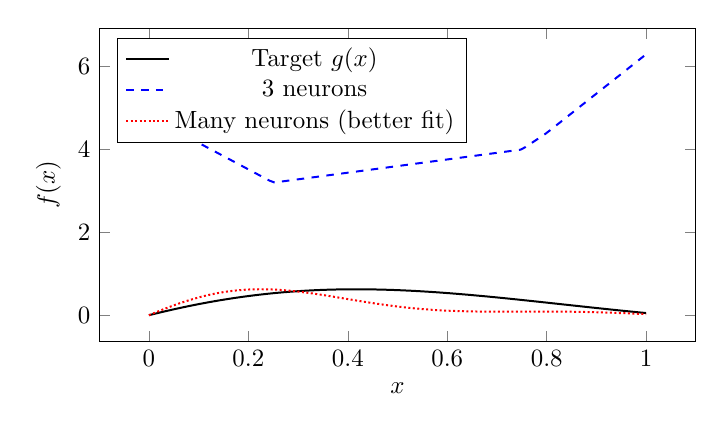
\begin{tikzpicture}[scale=0.9]
        \begin{axis}[
            xlabel=$x$,
            ylabel=$f(x)$,
            domain=0:1,
            samples=100,
            width=10cm,
            height=6cm,
            legend pos=north west
        ]
            % Target function
            \addplot[thick, black] {sin(deg(3*x)) * exp(-x)};
            \addlegendentry{Target $g(x)$}
            % Approximation with 3 neurons (staircase-like)
            \addplot[thick, blue, dashed] {max(0, 8*x - 2) + max(0, -8*x + 6)*0.8 + max(0, 5*x - 4)*0.3};
            \addlegendentry{3 neurons}
            % Approximation with more neurons
            \addplot[thick, red, densely dotted] {0.5*sin(deg(3*x))*exp(-x) + 0.3*sin(deg(6*x))*exp(-x) + 0.2*sin(deg(9*x))*exp(-x)};
            \addlegendentry{Many neurons (better fit)}
        \end{axis}
    \end{tikzpicture}
    \caption[Intuition behind universal approximation]{Each neuron contributes a ``bump'' or ``step.'' More neurons yield finer approximations of the target function.}
    \label{fig:uat_intuition}
\end{figure}

\subsection{Caveats and Practical Implications}

The universal approximation theorem is an \textbf{existence} result, not a \textbf{constructive} one. It tells us that a suitable network \emph{exists} but says nothing about:
\begin{enumerate}
    \item \textbf{How many neurons are needed}---the bound is astronomically loose for high-dimensional functions.
    \item \textbf{Whether gradient descent can find it}---the optimization landscape may have bad local minima.
    \item \textbf{Whether deeper networks are more efficient}---Cybenko's and Hornik's results apply to single hidden layers, but depth provides \emph{exponential} efficiency gains for compositional functions (see Montufar et al., 2014).
\end{enumerate}

In practice, deep networks (many layers, moderate width) vastly outperform shallow, wide networks. The key insight is that depth enables \textbf{hierarchical feature composition}---each layer builds increasingly abstract representations.

\section{Historical Development of Activation Functions}

Understanding the history of activation functions illuminates why certain choices became dominant and how the field evolved:

\begin{table}[ht]
    \centering
    \caption{Historical Timeline of Activation Function Development}
    \begin{tabular}{L{2cm} L{3cm} L{5.5cm} L{3cm}}
        \toprule
        \textbf{Year} & \textbf{Function} & \textbf{Context \& Motivation} & \textbf{Key Reference} \\
        \midrule
        1943 & Threshold (step) & McCulloch--Pitts neuron & McCulloch \& Pitts \\
        1957 & Perceptron & Linear threshold unit & Rosenblatt \\
        1960 & Adaline & Linear activation + sign & Widrow \& Hoff \\
        1986 & Sigmoid & Differentiable, backpropagation & Rumelhart et al. \\
        1991 & Tanh & Zero-centered alternative & \\
        1998 & ReLU & Biological inspiration & Hahnloser et al. \\
        2010 & Softmax & Probabilistic multi-class & \\
        2011 & ReLU (revival) & AlexNet: avoids vanishing gradients & \cite{krizhevsky2012imagenet} \\
        2015 & ELU, SELU & Smooth negative region & Clevert et al. \\
        2015 & PReLU & Learnable negative slope & He et al. \\
        2016 & Swish/SiLU & Self-gated, non-monotonic & Ramachandran et al. \\
        2016 & GELU & Probabilistic gating & Hendrycks \& Gimpel \\
        2019 & Mish & Self-regularized & Misra \\
        2022 & StarReLU & Efficient for transformers & Maulik et al. \\
        \bottomrule
    \end{tabular}
\end{table}

The story of ReLU's rise is particularly instructive. Before 2012, sigmoid and tanh were the standard choices. However, in deep networks, these saturating functions caused \textbf{vanishing gradients}---the gradient through a product of $L$ sigmoid derivatives is at most $(1/4)^L$, which becomes negligible for $L > 10$. The breakthrough of AlexNet \cite{krizhevsky2012imagenet} demonstrated that ReLU's non-saturating nature ($f'(x) = 1$ for $x > 0$) enables training of much deeper networks, fundamentally changing the field.

\section{Neural Network Neurons}

Before diving into activation functions, let us understand their role in a neuron.

A single artificial neuron computes:
\begin{equation}
y = f(\mathbf{w}^\top \mathbf{x} + b) = f\left(\sum_{i=1}^{n} w_i x_i + b\right)
\end{equation}
where:
\begin{itemize}
    \item $\mathbf{x} \in \mathbb{R}^n$ is the input vector
    \item $\mathbf{w} \in \mathbb{R}^n$ is the weight vector
    \item $b \in \mathbb{R}$ is the bias
    \item $f(\cdot)$ is the activation function
    \item $y \in \mathbb{R}$ is the output
\end{itemize}

\begin{figure}[htbp]
    \centering
    \begin{tikzpicture}[scale=0.9]
        % Input nodes
        \foreach \y/\label in {1/$x_1$, 2/$x_2$, 3/$\vdots$, 4/$x_n$} {
            \node[circle, draw=layer-input, fill=layer-input!30, minimum size=8mm] (x\y) at (0, 5-\y) {\label};
        }
        
        % Neuron
        \node[circle, draw=layer-hidden, fill=layer-hidden!30, minimum size=12mm, label=above:$f$] (neuron) at (4, 2.5) {$\sum + b$};
        
        % Output
        \node[circle, draw=layer-output, fill=layer-output!30, minimum size=8mm] (y) at (7, 2.5) {$y$};
        
        % Connections
        \foreach \i in {1,...,4} {
            \draw[->, thick] (x\i) -- (neuron);
        }
        \draw[->, thick] (neuron) -- (y);
        
        % Weights
        \foreach \y/\w in {1/$w_1$, 2/$w_2$, 3/, 4/$w_n$} {
            \node[right] at (0.7, 4.5-\y) {\w};
        }
    \end{tikzpicture}
    \caption[Singe neuron computation]{A single neuron computes a weighted sum followed by an activation function}
    \label{fig:neuron}
\end{figure}

\section{Linear Activation Functions}

While not technically ``activation functions'' in the practical sense, linear functions are sometimes used in output layers.

\subsection{Identity Function}

\begin{equation}
f(x) = x
\end{equation}

\begin{itemize}
    \item \textbf{Output range:} $(-\infty, \infty)$
    \item \textbf{Derivative:} $f'(x) = 1$
    \item \textbf{Use case:} Regression output layer
    \item \textbf{Not recommended:} Hidden layers (makes the network linear)
\end{itemize}

\section{Sigmoid Family}

The sigmoid family of activation functions squash their input into the range $(0, 1)$, making them useful for binary classification output layers.

\subsection{Sigmoid (Logistic)}

\begin{equation}
\sigma(x) = \frac{1}{1 + e^{-x}} = \frac{e^x}{e^x + 1}
\end{equation}

\begin{properties}[Properties of Sigmoid]
\begin{itemize}
    \item \textbf{Output range:} $(0, 1)$
    \item \textbf{Derivative:} $\sigma'(x) = \sigma(x)(1 - \sigma(x))$
    \item \textbf{Monotonically increasing}
    \item \textbf{Symmetric around 0.5}
    \item \textbf{Smooth and differentiable everywhere}
\end{itemize}
\end{properties}

\begin{figure}[htbp]
    \centering
    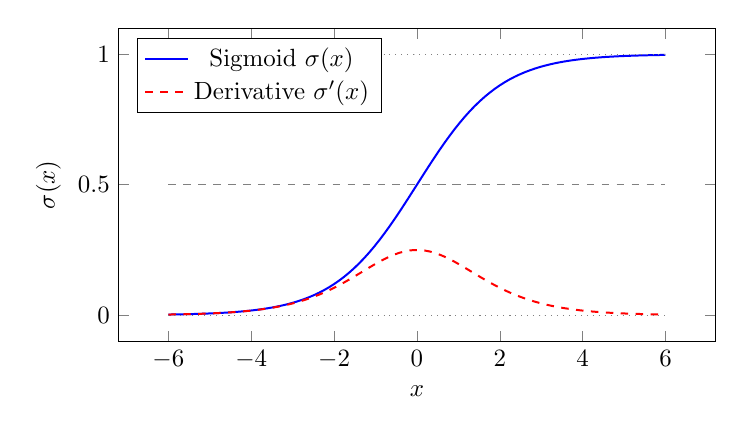
\begin{tikzpicture}[scale=0.9]
        \begin{axis}[
            xlabel=$x$,
            ylabel=$\sigma(x)$,
            domain=-6:6,
            samples=100,
            width=10cm,
            height=6cm,
            legend pos=north west
        ]
            \addplot[thick, blue] {1/(1 + exp(-x))};
            \addlegendentry{Sigmoid $\sigma(x)$}
            \addplot[thick, red, dashed] {exp(-x)/(1 + exp(-x))^2};
            \addlegendentry{Derivative $\sigma'(x)$}
            
            % Horizontal line at y=0.5
            \addplot[gray, dashed] {0.5};
            
            % Horizontal lines at y=0 and y=1
            \addplot[gray, dotted] {1};
            \addplot[gray, dotted] {0};
        \end{axis}
    \end{tikzpicture}
    \caption[Sigmoid function and its derivative]{The sigmoid function and its derivative}
    \label{fig:sigmoid}
\end{figure}

\begin{advantages}
    \item Smooth gradient
    \item Outputs can be interpreted as probabilities
    \item Historically widely used
\end{advantages}

\begin{disadvantages}
    \item \textbf{Vanishing gradient:} For large $|x|$, $\sigma'(x) \approx 0$
    \item \textbf{Not zero-centered:} Outputs are always positive
    \item \textbf{Exponential computation:} Slower than simpler functions
    \item \textbf{Saturation:} Sigmoid saturates at 0 and 1
\end{disadvantages}

\subsubsection{Mathematical Analysis: Why Sigmoid Causes Vanishing Gradients}

Consider an $L$-layer network where each layer uses sigmoid activation. During backpropagation, the gradient flowing through layer $l$ is multiplied by the derivative of each intermediate layer:
\begin{equation}
\frac{\partial \mathcal{L}}{\partial z_1} = \underbrace{\frac{\partial \mathcal{L}}{\partial z_L}}_{\text{output gradient}} \cdot \prod_{l=2}^{L} \underbrace{\frac{\partial a_l}{\partial z_l}}_{= \sigma'(z_l)} \cdot \underbrace{\frac{\partial z_l}{\partial a_{l-1}}}_{= \mathbf{W}_l}
\end{equation}

Since $\sigma'(z) = \sigma(z)(1-\sigma(z)) \leq \frac{1}{4}$ (maximum at $z=0$), the sigmoid derivative component alone provides a multiplicative factor of at most $(1/4)^{L-1}$:
\begin{equation}
\left\|\frac{\partial \mathcal{L}}{\partial z_1}\right\| \leq \left(\frac{1}{4}\right)^{L-1} \cdot \prod_{l=2}^{L} \|\mathbf{W}_l\| \cdot \left\|\frac{\partial \mathcal{L}}{\partial z_L}\right\|
\end{equation}

For a 50-layer network: $(1/4)^{49} \approx 10^{-30}$. Even with moderate weight norms, the gradient effectively vanishes. This mathematical analysis explains why sigmoid networks deeper than a few layers were essentially untrainable before alternative activation functions were adopted.

\subsubsection{Derivative Derivation}

Starting from $\sigma(x) = \frac{1}{1 + e^{-x}}$:
\begin{align}
\sigma'(x) &= \frac{d}{dx}\left((1 + e^{-x})^{-1}\right) = (1 + e^{-x})^{-2} \cdot e^{-x} \\
&= \frac{1}{1 + e^{-x}} \cdot \frac{e^{-x}}{1 + e^{-x}} \\
&= \sigma(x) \cdot (1 - \sigma(x))
\end{align}
This elegant form means the gradient can be computed directly from the output, without evaluating the exponential again. The maximum value $\sigma'(0) = 0.25$ occurs at $x = 0$.

\begin{example}[Sigmoid in Binary Classification]
For binary classification, the sigmoid output can be interpreted as:
\begin{equation}
P(y=1|\mathbf{x}) = \sigma(\mathbf{w}^\top \mathbf{x} + b)
\end{equation}
The cross-entropy loss with sigmoid is:
\begin{equation}
\mathcal{L} = -[y \log \hat{y} + (1-y) \log(1-\hat{y})]
\end{equation}
where $\hat{y} = \sigma(\mathbf{w}^\top \mathbf{x} + b)$.
\end{example}

\subsection{Hyperbolic Tangent (Tanh)}

\begin{equation}
\tanh(x) = \frac{e^x - e^{-x}}{e^x + e^{-x}} = 2\sigma(2x) - 1
\end{equation}

\begin{properties}[Properties of Tanh]
\begin{itemize}
    \item \textbf{Output range:} $(-1, 1)$
    \item \textbf{Derivative:} $\tanh'(x) = 1 - \tanh^2(x)$
    \item \textbf{Zero-centered output}
    \item \textbf{Monotonically increasing}
\end{itemize}
\end{properties}

\begin{figure}[htbp]
    \centering
    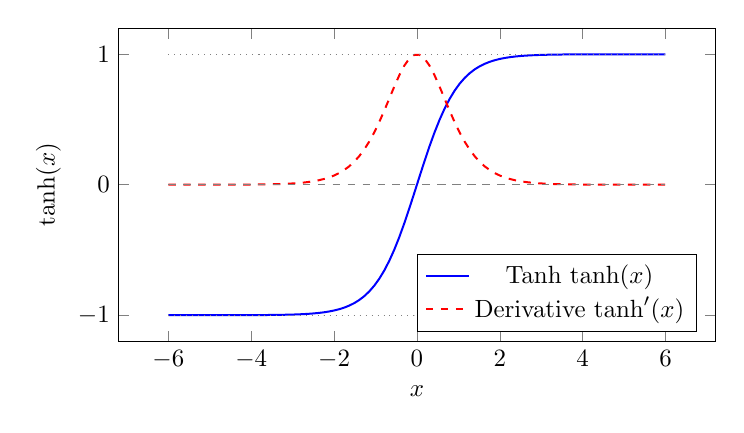
\begin{tikzpicture}[scale=0.9]
        \begin{axis}[
            xlabel=$x$,
            ylabel=$\tanh(x)$,
            domain=-6:6,
            samples=100,
            width=10cm,
            height=6cm,
            legend pos=south east
        ]
            \addplot[thick, blue] {tanh(x)};
            \addlegendentry{Tanh $\tanh(x)$}
            \addplot[thick, red, dashed] {1/(cosh(x)^2)};
            \addlegendentry{Derivative $\tanh'(x)$}
            
            % Horizontal lines
            \addplot[gray, dashed] {0};
            \addplot[gray, dotted] {1};
            \addplot[gray, dotted] {-1};
        \end{axis}
    \end{tikzpicture}
    \caption[Tanh function and its derivative]{The tanh function and its derivative}
    \label{fig:tanh}
\end{figure}

\begin{advantages}
    \item Zero-centered output (stronger gradients)
    \item Stronger gradients than sigmoid
    \item Outputs in $(-1, 1)$, often better for hidden layers
\end{advantages}

\begin{disadvantages}
    \item \textbf{Vanishing gradient:} Still present for large $|x|$
    \item \textbf{Exponential computation}
    \item \textbf{Saturation at $\pm 1$}
\end{disadvantages}

\section{Rectified Linear Unit (ReLU) Family}

The ReLU family has become the dominant choice for hidden layers in modern deep learning due to their computational efficiency and effectiveness in training deep networks.

\subsection{ReLU}

\begin{equation}
\text{ReLU}(x) = \max(0, x) = 
\begin{cases}
x & \text{if } x > 0 \\
0 & \text{if } x \leq 0
\end{cases}
\end{equation}

\begin{properties}[Properties of ReLU]
\begin{itemize}
    \item \textbf{Output range:} $[0, \infty)$
    \item \textbf{Derivative:} 
    \begin{equation}
    \text{ReLU}'(x) = 
    \begin{cases}
    1 & \text{if } x > 0 \\
    0 & \text{if } x \leq 0
    \end{cases}
    \end{equation}
    \item \textbf{Computationally efficient}
    \item \textbf{Sparse activation}
\end{itemize}
\end{properties}

\begin{figure}[htbp]
    \centering
    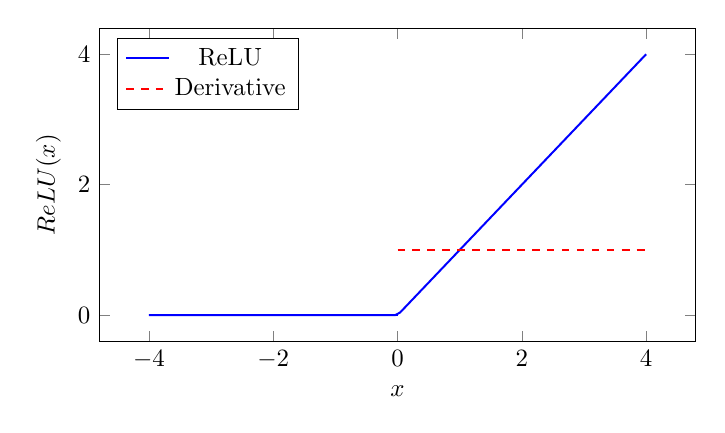
\begin{tikzpicture}[scale=0.9]
        \begin{axis}[
            xlabel=$x$,
            ylabel=$\text{ReLU}(x)$,
            domain=-4:4,
            samples=100,
            width=10cm,
            height=6cm,
            legend pos=north west
        ]
            \addplot[thick, blue] {max(0, x)};
            \addlegendentry{ReLU}
            \addplot[thick, red, dashed, domain=0:4] {1};
            \addlegendentry{Derivative}
            
            % Vertical line at x=0
            \addplot[const plot, thick, blue, domain=-4:0] {0};
        \end{axis}
    \end{tikzpicture}
    \caption[ReLU function and its derivative]{The ReLU function and its derivative}
    \label{fig:relu}
\end{figure}

\begin{advantages}
    \item \textbf{Very fast computation}
    \item \textbf{Reduces vanishing gradient problem} for positive activations
    \item \textbf{Sparse representations:} Not all neurons activate simultaneously
    \item \textbf{Excellent empirical performance} in deep networks
    \item \textbf{Biological plausibility}
\end{advantages}

\subsubsection{Why ReLU Prevents Vanishing Gradients: Mathematical Analysis}

The key advantage of ReLU over sigmoid is its \textbf{non-saturating} nature. For any neuron with a positive pre-activation $z_l > 0$:
\begin{equation}
\text{ReLU}'(z_l) = 1 \quad \text{(no attenuation)}
\end{equation}

In a deep network with ReLU activations, the gradient through the ``active'' path is:
\begin{equation}
\frac{\partial \mathcal{L}}{\partial z_1} = \frac{\partial \mathcal{L}}{\partial z_L} \cdot \prod_{l=2}^{L} \mathbf{1}_{\{z_l > 0\}} \cdot \mathbf{W}_l
\end{equation}
The indicator $\mathbf{1}_{\{z_l > 0\}}$ is either 0 or 1---there is no exponential decay. If roughly half the neurons are active at each layer, the gradient magnitude is:
\begin{equation}
\left\|\frac{\partial \mathcal{L}}{\partial z_1}\right\| \approx \left(\frac{1}{2}\right)^{L-1} \cdot \prod_{l=2}^{L} \|\mathbf{W}_l\| \cdot \left\|\frac{\partial \mathcal{L}}{\partial z_L}\right\|
\end{equation}

While the factor $(1/2)^{L-1}$ still decays exponentially, in practice this is mitigated by:
\begin{itemize}
    \item \textbf{He initialization} \cite{he2015delving}: Setting weight variance to $2/n_{\text{in}}$ compensates for the expected fraction of inactive neurons.
    \item \textbf{Residual connections} \cite{he2016deep}: Skip connections provide an alternative gradient path that bypasses multiplicative attenuation entirely (Chapter~6).
    \item \textbf{Batch normalization} \cite{ioffe2015batch}: Stabilizes the distribution of activations, keeping them in the non-saturated regime.
\end{itemize}

\subsubsection{ReLU, Sparsity, and Biological Motivation}

ReLU's $\max(0, x)$ operation creates sparse activations: for typical initialization, roughly 50\% of neurons output zero. This sparsity has several benefits:
\begin{enumerate}
    \item \textbf{Information disentanglement:} Sparse representations tend to be more interpretable and robust (similar to sparse coding in neuroscience).
    \item \textbf{Efficiency:} Zero-valued neurons contribute nothing to downstream computation, enabling hardware optimization.
    \item \textbf{Biological plausibility:} Biological neurons exhibit a threshold behavior---they fire only when input exceeds a threshold. ReLU captures this qualitatively, unlike the smooth sigmoid.
\end{enumerate}

\begin{disadvantages}
    \item \textbf{Dying ReLU problem:} Neurons can ``die'' if they always output zero
    \item \textbf{Not zero-centered}
    \item \textbf{Unbounded output}
\end{disadvantages}

\begin{note}[Dying ReLU Problem]
If a neuron's weights are updated such that $\mathbf{w}^\top \mathbf{x} + b \leq 0$ for all inputs, the neuron will output zero forever. This is called the ``dying ReLU'' or ``dead neuron'' problem. The neuron stops learning because the gradient is zero when the input is negative.

Solutions include:
\begin{itemize}
    \item Leaky ReLU
    \item PReLU
    \item ELU
    \item Proper weight initialization
    \item Lower learning rates
\end{itemize}
\end{note}

\subsection{Leaky ReLU}

\begin{equation}
\text{LeakyReLU}(x) = 
\begin{cases}
x & \text{if } x > 0 \\
\alpha x & \text{if } x \leq 0
\end{cases}
= \max(0, x) + \alpha \min(0, x)
\end{equation}
where $\alpha$ is a small positive constant (typically $\alpha = 0.01$).

\begin{properties}[Properties of Leaky ReLU]
\begin{itemize}
    \item \textbf{Output range:} $(-\infty, \infty)$
    \item \textbf{Derivative:} 
    \begin{equation}
    \text{LeakyReLU}'(x) = 
    \begin{cases}
    1 & \text{if } x > 0 \\
    \alpha & \text{if } x \leq 0
    \end{cases}
    \end{equation}
    \item \textbf{Small negative values allowed}
\end{itemize}
\end{properties}

\begin{advantages}
    \item \textbf{No dying ReLU problem}
    \item \textbf{Allows small negative gradients}
    \item \textbf{Approximately zero-centered}
\end{advantages}

\begin{disadvantages}
    \item Hyperparameter $\alpha$ needs tuning
    \item Performance may not be significantly better than ReLU
\end{disadvantages}

\subsection{Parametric ReLU (PReLU)}

\begin{equation}
\text{PReLU}(x) = 
\begin{cases}
x & \text{if } x > 0 \\
\alpha x & \text{if } x \leq 0
\end{cases}
\end{equation}
where $\alpha$ is a learnable parameter (can be per channel).

\begin{note}
PReLU allows the network to learn the optimal slope for negative values, potentially improving performance.
\end{note}

\subsection{Exponential Linear Unit (ELU)}

\begin{equation}
\text{ELU}(x) = 
\begin{cases}
x & \text{if } x > 0 \\
\alpha(e^x - 1) & \text{if } x \leq 0
\end{cases}
\end{equation}
where $\alpha > 0$ is a hyperparameter.

\begin{properties}[Properties of ELU]
\begin{itemize}
    \item \textbf{Output range:} $(-\alpha, \infty)$
    \item \textbf{Smooth for $x < 0$}
    \item \textbf{Negative values bring mean closer to zero}
\end{itemize}
\end{properties}

\begin{figure}[htbp]
    \centering
    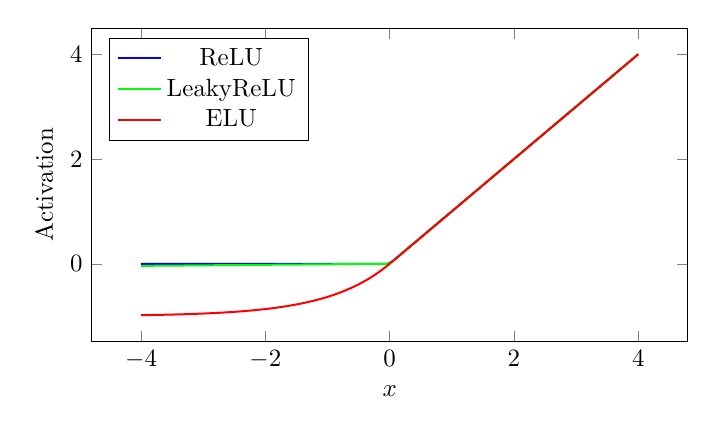
\begin{tikzpicture}[scale=0.9]
        \begin{axis}[
            xlabel=$x$,
            ylabel=Activation,
            domain=-4:4,
            samples=100,
            width=10cm,
            height=6cm,
            legend pos=north west
        ]
            \addplot[thick, blue] {max(0, x)};
            \addlegendentry{ReLU}
            \addplot[thick, green] {max(0, x) + 0.01*min(0, x)};
            \addlegendentry{LeakyReLU}
            \addplot[thick, red] {x > 0 ? x : 1.0*(exp(x) - 1)};
            \addlegendentry{ELU}
        \end{axis}
    \end{tikzpicture}
    \caption[Comparison of ReLU variants]{Comparison of ReLU and its variants}
    \label{fig:relu_variants}
\end{figure}

\begin{advantages}
    \item \textbf{No dying ReLU problem}
    \item \textbf{Outputs closer to zero mean}
    \item \textbf{Smoother gradients}
\end{advantages}

\begin{disadvantages}
    \item Exponential computation for negative values
    \item Slower forward pass
\end{disadvantages}

\subsection{Swish / SiLU}

\begin{equation}
\text{Swish}(x) = x \cdot \sigma(x) = \frac{x}{1 + e^{-x}}
\end{equation}

Proposed by Ramachandran et al. (2017), Swish often outperforms ReLU in deeper networks.

\begin{properties}[Properties of Swish]
\begin{itemize}
    \item \textbf{Output range:} Approximately $(-0.31, \infty)$
    \item \textbf{Self-gated}
    \item \textbf{Non-monotonic} (dip for small negative values)
    \item \textbf{Derivative:} $\text{Swish}'(x) = \sigma(x) + x \cdot \sigma(x)(1 - \sigma(x)) = \text{Swish}(x) + \sigma(x)(1 - \text{Swish}(x))$
\end{itemize}
\end{properties}

\begin{figure}[htbp]
    \centering
    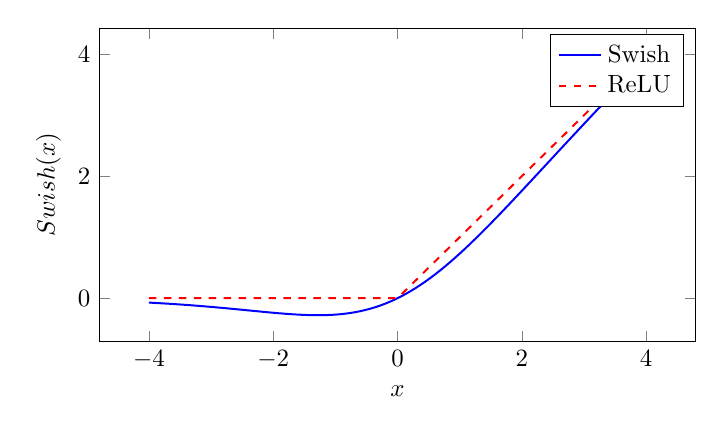
\begin{tikzpicture}[scale=0.9]
        \begin{axis}[
            xlabel=$x$,
            ylabel=$\text{Swish}(x)$,
            domain=-4:4,
            samples=100,
            width=10cm,
            height=6cm
        ]
            \addplot[thick, blue] {x / (1 + exp(-x))};
            \addlegendentry{Swish}
            \addplot[thick, red, dashed] {max(0, x)};
            \addlegendentry{ReLU}
        \end{axis}
    \end{tikzpicture}
    \caption[Swish activation function]{Swish vs ReLU}
    \label{fig:swish}
\end{figure}

\subsection{Mish}

Proposed by Misra (2019) \cite{misra2019mish}, Mish is a self-regularized, non-monotonic activation function:
\begin{equation}
\text{Mish}(x) = x \cdot \tanh(\text{softplus}(x)) = x \cdot \tanh(\ln(1 + e^x))
\end{equation}

\begin{properties}[Properties of Mish]
\begin{itemize}
    \item \textbf{Output range:} Approximately $(-0.308, \infty)$ (bounded below, unbounded above)
    \item \textbf{Non-monotonic:} Similar to Swish, dips slightly for negative $x$
    \item \textbf{Smooth everywhere:} Infinitely differentiable ($C^\infty$)
    \item \textbf{Self-regularizing:} The non-monotonic shape acts as an implicit regularizer
\end{itemize}
\end{properties}

The derivative is:
\begin{equation}
\text{Mish}'(x) = \frac{e^x \cdot (4(e^x + 2)) + 4x \cdot e^{2x} + 2 \cdot e^{3x} + x \cdot e^{4x} + 2}{(2e^x + 2)^2}
\end{equation}

While the derivative is complex, the key insight is that Mish maintains a positive gradient throughout (like ReLU) but with a smoother, bounded gradient for negative inputs that provides gentle regularization. Empirically, Mish consistently matches or outperforms ReLU and Swish across image classification benchmarks (ImageNet, CIFAR-10/100) and object detection tasks.

\begin{advantages}
    \item Stronger performance than ReLU/Swish on vision tasks
    \item Smooth, non-monotonic shape provides implicit regularization
    \item No additional hyperparameters
\end{advantages}

\begin{disadvantages}
    \item More expensive computation ($\tanh$ + softplus)
    \item Complex derivative formula
\end{disadvantages}

\subsection{StarReLU}

Introduced by Maulik et al. (2024) \cite{maulik2024starrelu}, StarReLU is a self-gated activation function specifically designed for transformers:
\begin{equation}
\text{StarReLU}(x) = s \cdot \text{ReLU}(x)^2 + \beta
\end{equation}
where $s$ and $\beta$ are learnable parameters (initialized to $s = 1, \beta = 0$).

\textbf{Motivation:} In transformers, the computational bottleneck is the activation function applied to every element of the $N \times d$ hidden state tensor. StarReLU's quadratic form $\text{ReLU}(x)^2$ is simpler than GELU/Swish (no $\tanh$ or $\sigma$) while providing:
\begin{itemize}
    \item \textbf{Self-gating:} The squaring operation naturally gates negative inputs to zero.
    \item \textbf{Learnable scale and shift:} $s$ and $\beta$ adapt the activation range.
    \item \textbf{Computational efficiency:} 60\% fewer FLOPs than GELU in transformer blocks, with no accuracy loss.
\end{itemize}

StarReLU represents the trend of designing activation functions that are \textbf{hardware-aware}---exploiting the fact that simple operations (multiply, add) are far cheaper than transcendental functions (exp, tanh, erf) on modern hardware.

\subsection{GELU (Gaussian Error Linear Unit)}

\begin{equation}
\text{GELU}(x) = x \cdot \Phi(x)
\end{equation}
where $\Phi(x)$ is the CDF of the standard normal distribution:
\begin{equation}
\Phi(x) = \frac{1}{2}\left[1 + \text{erf}\left(\frac{x}{\sqrt{2}}\right)\right]
\end{equation}

A computationally efficient approximation:
\begin{equation}
\text{GELU}(x) \approx \frac{x}{2} \cdot \left(1 + \tanh\left(\sqrt{\frac{2}{\pi}}\left(x + 0.044715x^3\right)\right)\right)
\end{equation}

GELU is used in BERT, GPT, and many transformer architectures.

\subsubsection{Probabilistic Interpretation: GELU, Dropout, and the Gaussian CDF}

The GELU function has a deep probabilistic interpretation that connects it to dropout \cite{clark2022unified}. Consider a stochastic neuron where the input $x$ is multiplied by a random Bernoulli mask $m \sim \text{Bernoulli}(\Phi(x))$:
\begin{equation}
y = x \cdot m, \quad P(m = 1 \mid x) = \Phi(x)
\end{equation}
The expected output of this stochastic neuron is:
\begin{equation}
\mathbb{E}[y \mid x] = x \cdot \Phi(x) = \text{GELU}(x)
\end{equation}

\textbf{Key insight:} GELU is the \emph{deterministic expectation} of a stochastically gated neuron where the gate probability equals the Gaussian CDF. This provides a unified view:
\begin{itemize}
    \item \textbf{Dropout} randomly zeroes activations with probability $p$ (input-independent).
    \item \textbf{GELU} adaptively gates activations based on their magnitude (input-dependent).
    \item Both can be viewed as multiplicative noise, but GELU's noise is \emph{adaptive}---larger inputs are more likely to pass through.
\end{itemize}

This interpretation explains why GELU works so well in transformers: it provides a smooth, ``soft'' version of dropout that depends on the input magnitude, offering implicit regularization without the training instability of random dropout in attention mechanisms.

\subsubsection{Derivative of GELU}

From $\text{GELU}(x) = x\Phi(x)$, by the product rule:
\begin{equation}
\text{GELU}'(x) = \Phi(x) + x\phi(x)
\end{equation}
where $\phi(x) = \frac{1}{\sqrt{2\pi}}e^{-x^2/2}$ is the standard normal PDF. Note that $\text{GELU}'(x) > 0$ for all $x$ (the function is strictly increasing) but $\text{GELU}'(x) < 1$ (unlike ReLU), providing natural gradient scaling.

\begin{properties}[Properties of GELU]
\begin{itemize}
    \item \textbf{Stochastic regularizer} when used with dropout
    \item \textbf{Nonlinear in all regions}
    \item \textbf{Approximately equal to: $0.5x(1 + \tanh(\sqrt{2/\pi}(x + 0.044715x^3)))$}
    \item \textbf{Zero-centered output}
\end{itemize}
\end{properties}

\begin{advantages}
    \item State-of-the-art performance in transformers
    \item Combines benefits of ReLU and dropout
    \item Smooth and non-monotonic
\end{advantages}

\section{Special Activation Functions}

\subsection{Softmax}

\begin{equation}
\text{softmax}(x_i) = \frac{e^{x_i}}{\sum_{j=1}^{K} e^{x_j}} \quad \text{for } i = 1, \ldots, K
\end{equation}

Softmax is used for multi-class classification output layers.

\begin{properties}[Properties of Softmax]
\begin{itemize}
    \item \textbf{Output range:} Each output in $(0, 1)$
    \item \textbf{Sum constraint:} $\sum_i \text{softmax}(x_i) = 1$
    \item \textbf{Probabilistic interpretation}
    \item \textbf{Shift invariant:} $\text{softmax}(x + c) = \text{softmax}(x)$ for any constant $c$
\end{itemize}
\end{properties}

\begin{advantages}
    \item Outputs are valid probability distributions
    \item Enables cross-entropy loss optimization
    \item Handles multi-class classification naturally
\end{advantages}

\begin{disadvantages}
    \item Only used in output layers (not hidden layers)
    \item Can saturate when logits are very large
\end{disadvantages}

\begin{note}[Softmax in Practice]
For numerical stability, implement softmax as:
\begin{equation}
\text{softmax}(x_i) = \frac{e^{x_i - \max(x)}}{\sum_j e^{x_j - \max(x)}}
\end{equation}
This subtracts the maximum value to prevent overflow in the exponential.
\end{note}

\section{Choosing an Activation Function}

The choice of activation function depends on the specific task and network architecture. Here are general guidelines:

\begin{table}[ht]
    \centering
    \caption{Activation Function Selection Guide}
    \begin{tabular}{L{3cm} L{5cm} L{4cm}}
        \toprule
        \textbf{Layer Type} & \textbf{Recommended Functions} & \textbf{Notes} \\
        \midrule
        \textbf{Hidden (General)} & ReLU, GELU & ReLU is the default choice \\
        \textbf{Hidden (Deep)} & ReLU, GELU, ELU & Avoid sigmoid/tanh in deep networks \\
        \textbf{Hidden (CNN)} & ReLU, GELU & LeakyReLU for medical imaging \\
        \textbf{Hidden (RNN)} & Tanh & Often default for RNNs \\
        \textbf{Hidden (Transformer)} & GELU & Used in BERT, GPT, etc. \\
        \textbf{Output (Binary)} & Sigmoid & For probability output \\
        \textbf{Output (Multi-class)} & Softmax & For probability distribution \\
        \textbf{Output (Regression)} & Identity / None & For unbounded output \\
        \textbf{Output (Bounded)} & Sigmoid, Tanh & For $[0,1]$ or $[-1,1]$ output \\
        \bottomrule
    \end{tabular}
\end{table}

\begin{figure}[htbp]
    \centering
    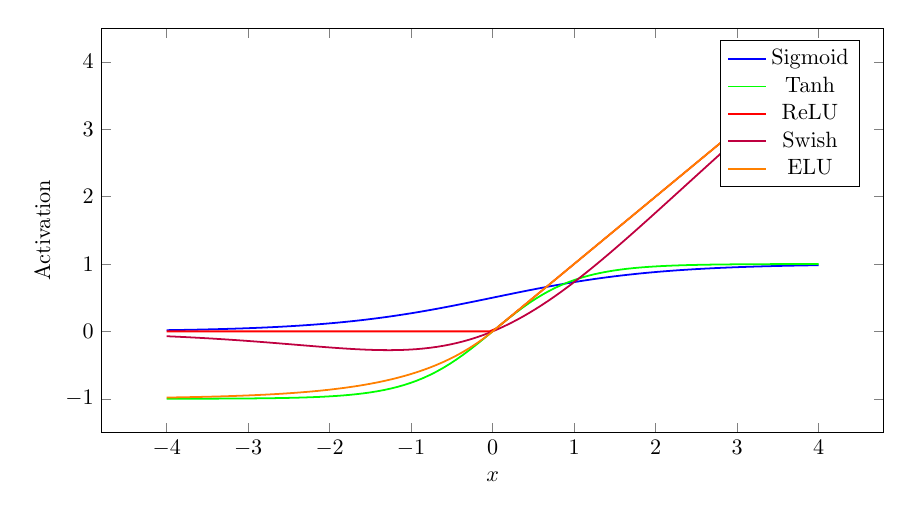
\begin{tikzpicture}[scale=0.8]
        \begin{axis}[
            xlabel=$x$,
            ylabel=Activation,
            domain=-4:4,
            samples=100,
            width=14cm,
            height=8cm,
            legend pos=north east
        ]
            \addplot[thick, blue] {1/(1 + exp(-x))};
            \addlegendentry{Sigmoid}
            \addplot[thick, green] {tanh(x)};
            \addlegendentry{Tanh}
            \addplot[thick, red] {max(0, x)};
            \addlegendentry{ReLU}
            \addplot[thick, purple] {x / (1 + exp(-x))};
            \addlegendentry{Swish}
            \addplot[thick, orange] {x > 0 ? x : 1.0*(exp(x) - 1)};
            \addlegendentry{ELU}
        \end{axis}
    \end{tikzpicture}
    \caption[Comparison of activation functions]{Comparison of various activation functions}
    \label{fig:activation_comparison}
\end{figure}

\section{Practical Considerations}

\subsection{Weight Initialization}

Different activation functions work best with appropriate weight initialization:

\begin{itemize}
    \item \textbf{Sigmoid/Tanh:} Xavier/Glorot initialization ($\mathcal{N}(0, \sqrt{2/(n_{in} + n_{out})})$)
    \item \textbf{ReLU (and variants):} He initialization ($\mathcal{N}(0, \sqrt{2/n_{in})})$)
    \item \textbf{GELU:} He initialization works well
\end{itemize}

See Chapter 7 on Optimization for more details.

\subsection{Batch Normalization with Activations}

When using batch normalization, the activation function typically comes \textbf{after} batch norm:
\begin{equation}
\mathbf{y} = f(\text{BN}(\mathbf{W}\mathbf{x} + \mathbf{b}))
\end{equation}

This ordering was popularized by the original BatchNorm paper and is now standard practice.

\section{Implementation in PyTorch}

\begin{code}
    \captionof{listing}{Activation Functions in PyTorch}
    \label{code:activations_pytorch}
\begin{lstlisting}[language=python]
import torch
import torch.nn as nn

# Common activations
relu = nn.ReLU()
leaky_relu = nn.LeakyReLU(0.01)  # slope for negative values
prelu = nn.PReLU()  # learnable slope
elu = nn.ELU(alpha=1.0)
selu = nn.SELU()  # Self-Normalizing Neural Networks
gelu = nn.GELU()  # Used in Transformers
silu = nn.SiLU()  # Same as Swish
sigmoid = nn.Sigmoid()
tanh = nn.Tanh()
softmax = nn.Softmax(dim=1)

# Example usage
x = torch.randn(32, 128)  # batch of 32, 128 features
y = relu(x)  # Apply ReLU

# Softmax with dimension specification
logits = torch.randn(32, 10)  # 10 classes
probs = softmax(dim=1)(logits)

# GELU in transformers
transformer_layer = nn.TransformerEncoderLayer(
    d_model=512, 
    nhead=8,
    activation='gelu'  # or use nn.GELU() directly
)
\end{lstlisting}
\end{code}

\section{Chapter Summary}

\begin{enumerate}
    \item \textbf{Activation functions introduce nonlinearity} into neural networks, enabling them to learn complex patterns.
    
    \item \textbf{Sigmoid and Tanh} squash inputs to bounded ranges but suffer from vanishing gradients.
    
    \item \textbf{ReLU} is computationally efficient and reduces vanishing gradients but can suffer from dying neurons.
    
    \item \textbf{Variants like Leaky ReLU, PReLU, and ELU} address the dying ReLU problem.
    
    \item \textbf{GELU} has become popular in transformer architectures.
    
    \item \textbf{Softmax} is used for multi-class classification output layers.
    
    \item \textbf{Choice depends on} task, architecture, and training stability.
\end{enumerate}

\begin{table}[ht]
    \centering
    \caption{Activation Function Quick Reference}
    \begin{tabular}{L{2.5cm} L{2.5cm} L{2cm} L{3cm}}
        \toprule
        \textbf{Function} & \textbf{Formula} & \textbf{Range} & \textbf{Common Use} \\
        \midrule
        Sigmoid & $1/(1+e^{-x})$ & $(0,1)$ & Binary output \\
        Tanh & $(e^x-e^{-x})/(e^x+e^{-x})$ & $(-1,1)$ & RNN, rarely CNN \\
        ReLU & $\max(0,x)$ & $[0,\infty)$ & Default hidden \\
        Leaky ReLU & $\max(\alpha x, x)$ & $(-\infty,\infty)$ & Prevent dying \\
        ELU & $x$ if $x>0$, else $\alpha(e^x-1)$ & $(-\alpha,\infty)$ & Better gradients \\
        GELU & $x \cdot \Phi(x)$ & varies & Transformers \\
        Softmax & $e^{x_i}/\sum e^{x_j}$ & $(0,1)^K$ & Multi-class output \\
        \bottomrule
    \end{tabular}
\end{table}

\section{Further Reading}

\begin{itemize}
    \item \cite{hornik1991approximation} - Universal Approximation Theorem: theoretical foundations
    \item Ramachandran et al., ``Searching for Activation Functions'' (2017) - Systematic comparison of activation functions
    \item Hendrycks and Gimpel, ``Gaussian Error Linear Units (GELU)'' (2016) - Introduction of GELU
    \item \cite{clark2022unified} - Unified view of GELU activation and dropout
    \item Clevert et al., ``Fast and Accurate Deep Network Learning by Exponential Linear Units (ELUs)'' (2015)
    \item \cite{misra2019mish} - Mish: A self-regularized non-monotonic neural activation function
    \item \cite{maulik2024starrelu} - StarReLU: Efficient self-gated activation for transformers
    \item Goodfellow et al., ``Deep Learning'' Chapter 6
    \item \cite{he2015delving} - Delving deep into rectifiers: He initialization
\end{itemize}

\section{Exercises}

\begin{enumerate}
    \item \textbf{Gradient Analysis:} Compute the gradient of the ELU function for both positive and negative inputs.
    
    \item \textbf{Comparison:} Plot the activation functions covered in this chapter and their derivatives using Python/Matplotlib.
    
    \item \textbf{Dying ReLU:} Implement a simple experiment to demonstrate the dying ReLU problem and show how LeakyReLU addresses it.
    
    \item \textbf{Numerical Stability:} Show why subtracting $\max(x)$ from logits before computing softmax improves numerical stability.
    
    \item \textbf{Custom Activation:} Design and implement a custom activation function that combines properties of ReLU and GELU. Test it on a simple image classification task.
    
    \item \textbf{Self-Normalization:} Research SELU (Scaled Exponential Linear Unit) and explain how it enables self-normalizing neural networks.
\end{enumerate}
